% TikZ version of the Marketing Analytics Ecosystem (Venn diagram)
% Clean version

\documentclass[tikz,border=10pt]{standalone}
\usepackage{tikz}
\usetikzlibrary{positioning,shapes,calc,fit,backgrounds}

% Define fonts if not available
\providecommand{\sffamily}{\familydefault}

\begin{document}

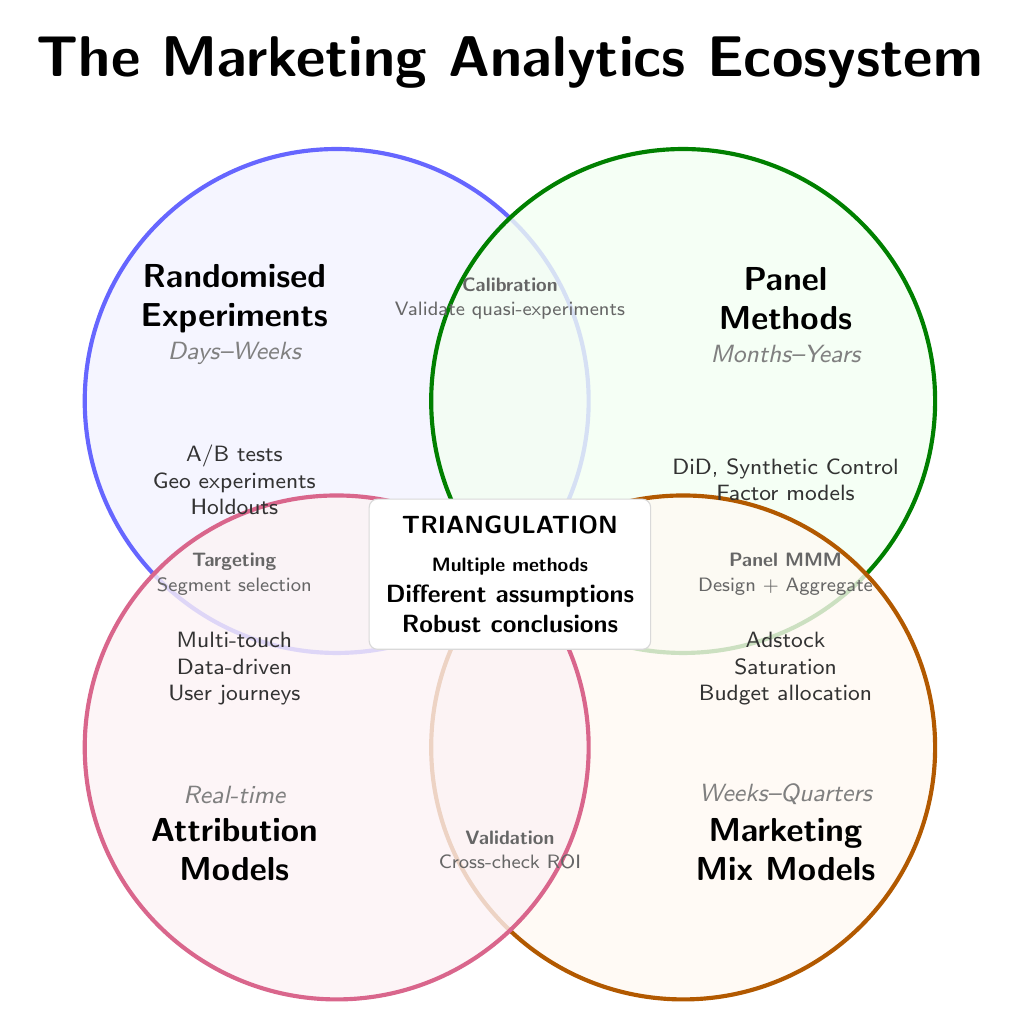
\begin{tikzpicture}[
    % Circle styles - lighter and cleaner
    exp/.style={fill=blue!5, draw=blue!60, line width=1.5pt, fill opacity=0.8},
    panel/.style={fill=green!5, draw=green!50!black, line width=1.5pt, fill opacity=0.8},
    mmm/.style={fill=orange!5, draw=orange!70!black, line width=1.5pt, fill opacity=0.8},
    attr/.style={fill=purple!5, draw=purple!60, line width=1.5pt, fill opacity=0.8},
    % Label styles
    pillar/.style={font=\bfseries\sffamily\large, align=center},
    timeline/.style={font=\sffamily\small\itshape, text=gray},
    detail/.style={font=\sffamily\footnotesize, align=center, text=black!80},
    intersection/.style={font=\sffamily\scriptsize, align=center, text=black!60},
    center/.style={font=\bfseries\sffamily\small, align=center},
]

% Define circle centers (wider spread)
\coordinate (exp-center) at (-2.2, 2.2);
\coordinate (panel-center) at (2.2, 2.2);
\coordinate (mmm-center) at (2.2, -2.2);
\coordinate (attr-center) at (-2.2, -2.2);
\def\radius{3.2}

% Draw the four overlapping circles
\begin{scope}[even odd rule]
    \draw[exp] (exp-center) circle (\radius);
    \draw[panel] (panel-center) circle (\radius);
    \draw[mmm] (mmm-center) circle (\radius);
    \draw[attr] (attr-center) circle (\radius);
\end{scope}

% Pillar labels (centered in non-overlapping regions)
\node[pillar] at (-3.5, 3.5) {Randomised\\Experiments};
\node[timeline] at (-3.5, 2.8) {Days--Weeks};

\node[pillar] at (3.5, 3.5) {Panel\\Methods};
\node[timeline] at (3.5, 2.8) {Months--Years};

\node[pillar] at (3.5, -3.5) {Marketing\\Mix Models};
\node[timeline] at (3.5, -2.8) {Weeks--Quarters};

\node[pillar] at (-3.5, -3.5) {Attribution\\Models};
\node[timeline] at (-3.5, -2.8) {Real-time};

% Details in non-overlapping regions (cleaner lists)
\node[detail] at (-3.5, 1.2) {A/B tests\\Geo experiments\\Holdouts};
\node[detail] at (3.5, 1.2) {DiD, Synthetic Control\\Factor models};
\node[detail] at (3.5, -1.2) {Adstock\\Saturation\\Budget allocation};
\node[detail] at (-3.5, -1.2) {Multi-touch\\Data-driven\\User journeys};

% Pairwise intersection labels (simplified)
\node[intersection] at (0, 3.5) {\textbf{Calibration}\\[1pt]Validate quasi-experiments};
\node[intersection] at (3.5, 0) {\textbf{Panel MMM}\\[1pt]Design + Aggregate};
\node[intersection] at (0, -3.5) {\textbf{Validation}\\[1pt]Cross-check ROI};
\node[intersection] at (-3.5, 0) {\textbf{Targeting}\\[1pt]Segment selection};

% Central triangulation region (cleaner box)
\node[center, fill=white, draw=gray!30, rounded corners=3pt, inner sep=6pt] at (0, 0) 
    {\textbf{TRIANGULATION}\\[3pt]\scriptsize Multiple methods\\Different assumptions\\Robust conclusions};

% Title
\node[font=\bfseries\huge\sffamily] at (0, 6.5) {The Marketing Analytics Ecosystem};

\end{tikzpicture}

\end{document}
